\documentclass[aspectratio=169]{beamer}
%\documentclass[handout]{beamer}

% language settings
%\usepackage{fontspec, polyglossia}
%\setdefaultlanguage{magyar}

% common packages
\usepackage{amsmath, multimedia, hyperref, color, multirow}
%\usepackage{graphicx}
\usepackage{pifont}

% TikZ
\usepackage{tikz}
\usetikzlibrary{arrows.meta, decorations.pathmorphing, decorations.pathreplacing, shapes.geometric,mindmap}
\usetikzlibrary{shapes.geometric,fadings,bayesnet}

% beamer styles
\mode<presentation>{
%\usetheme{Pittsburgh}
\usetheme{Boadilla}
\usecolortheme{beaver}
%\usecolortheme{seahorse}
%\usefonttheme{structureitalicserif}
\setbeamercovered{transparent}
}
\setbeamertemplate{blocks}[rounded][shadow=true]
\AtBeginSubsection[]{
  \begin{frame}<beamer>{Contents}
  \end{frame}
}
%\useoutertheme[]{tree}

% title, etc
%\title{Drug Repurposing to Alzheimer's Disease Using TWAS and the PPI Network}
\title{Omics Driven Drug Repurposing for Alzheimer's}
\author{Anjali Lathwal, Attila Jones}
\date{CTNS: Clinical \& Translational Neuroscience Section}

\begin{document}

\maketitle

\begin{frame}<1-7>[label=dream]{DREAM$^\ast$}{$^\ast$Drug Repurposing for Effective Alzheimer's Medicines}
\begin{columns}[t]
\begin{column}{0.4\textwidth}
\begin{enumerate}
\item<1-> collect AD genes\\
{\tiny risk ($\approx 100$) \emph{vs}.~assoc. ($\approx 10,000$)}
\begin{itemize}
\item<1> curated knowledge
\item<2> our AD gene discoveries
\item<3> public omic data
\item<4> association resources
\end{itemize}
\item<5-> prioritize all approved drugs
\begin{itemize}
\item<5> shared gene approach---Anjali
\item<6> network approach---Attila
\end{itemize}
\item<7-> validate
\begin{itemize}
\item \emph{in vitro} essays
\item pharmacoepidemiology
\end{itemize}
\end{enumerate}
\end{column}

\begin{column}{0.6\textwidth}

\includegraphics<1>[width=0.3\columnwidth]{figures/from-others/uniprot-logo.png}
\includegraphics<1>[width=0.3\columnwidth]{figures/from-others/amyco-logo.png}

\includegraphics<2>[width=0.8\columnwidth]{figures/from-others/jackson-APOE-Fig2c.png}

\only<2>{\tiny Roberts,..., Thambisetty 2021 Science Advances}

\includegraphics<3>[width=1.0\columnwidth]{figures/from-others/schwartzentruber-fig1b.png}

\only<3>{\tiny Schwartzentruber et al 2021 Nat Genet}

\includegraphics<5-6>[width=0.3\columnwidth]{figures/from-others/drugbank-logo.png}

\includegraphics<4>[width=0.5\columnwidth]{figures/from-others/disgenet-logo.png}

\includegraphics<5>[]{figures/by-me/repos-shared-gene/repos-shared-gene.pdf}

\includegraphics<6>[width=0.5\columnwidth]{figures/from-others/rual-2005-interactome-Fig2b.png}

\only<6>{\tiny The human interactome}

%\includegraphics<3>[width=0.2\columnwidth]{figures/from-others/gtex.png}
\end{column}
\end{columns}
\end{frame}

\begin{frame}[label=repurposing]{Drug repurposing}
\begin{columns}[t]
\begin{column}{0.5\textwidth}

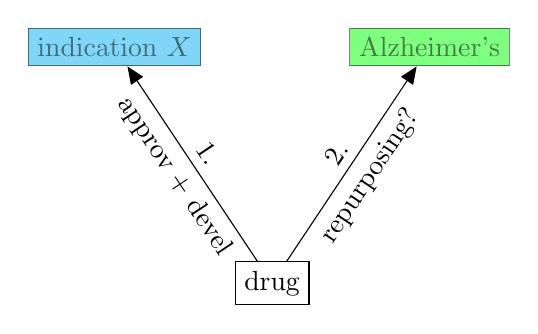
\begin{tikzpicture}
\path (0,0) node[draw] (drug) {drug}
	(-2,3) node[draw,fill=cyan,semitransparent] (ind) {indication $X$}
	( 2,3) node[draw,fill=green,semitransparent] (alz) {Alzheimer's};
\path[->] (drug) edge node[below,sloped,text width=3cm,text centered] {approv
	+ devel} node[above,sloped]
	{1.} (ind);
\path[->] (drug) edge node[below,sloped] {repurposing?} node[above,sloped]
	{2.} (alz);
\end{tikzpicture}
\end{column}

\begin{column}{0.5\textwidth}
\begin{enumerate}
	\item<2-> shared gene approach---Anjali\\
\includegraphics<2->[]{figures/by-me/repos-shared-gene/repos-shared-gene.pdf}
\normalsize
\item<3> network approach---Attila
\begin{description}
\footnotesize
\item[Guney,..., Barabási 2016] proximity
\item[Cheng,..., Barabási 2018] validation
\end{description}
\end{enumerate}
\end{column}
\end{columns}
\includegraphics<3>[]{figures/by-me/repos-network/repos-network.pdf}
\end{frame}

\begin{frame}
\begin{center}
	Anjali next
\end{center}
\end{frame}

\againframe<3>{repurposing}

\begin{frame}{Quantifying repurposing potential in a toy gene network}
\begin{columns}[t]
\begin{column}{0.5\textwidth}
disease gene set $S = \{$
{\tiny
\tikz{\node[white,circle,inner sep=1pt,fill=red] {B}}
\tikz{\node[white,circle,inner sep=1pt,fill=red] {D}}
\tikz{\node[white,rectangle,inner sep=2.5pt,fill=red] {E}}
}
$\}$

target gene set $T = \{$
{\tiny
\tikz{\node[white,rectangle,inner sep=2.5pt,fill=blue] {J}}
\tikz{\node[white,rectangle,inner sep=2.5pt,fill=red] {E}}
}
$\}$

\begin{enumerate}
\item<2-> raw distance
\begin{equation*}
d = \frac{1}{|T|}\sum_{t \in T} \min_{s \in S} d(s, t)
\end{equation*}
\item<3-> $z$-score
\begin{equation*}
z = \frac{d - \bar{d}_0}{s_0}
\end{equation*}
\item<4-> $p$-value
\begin{equation*}
p = \Pr(z \le Z)
\end{equation*}
\end{enumerate}
\end{column}

\footnotesize
\begin{column}{0.25\textwidth}

\includegraphics<1->[width=1\columnwidth]{../../../results/2021-06-14-proximity/toy-proximal-arrow.png}

\begin{eqnarray*}
\visible<2->{
d &=& \frac{1}{2} (0 + 1) = 0.5 \\ }
\visible<3->{
z &=& -0.454 \\ }
\visible<4->{
p &=& 0.324 \\ }
\end{eqnarray*}
\end{column}
\begin{column}{0.25\textwidth}

\includegraphics<5>[width=1\columnwidth]{../../../results/2021-06-14-proximity/toy-distal-arrow.png}

\visible<5>{
\begin{eqnarray*}
d &=& \frac{1}{2} (2 + 1) = 1.5 \\
z &=& 2.217 \\
p &=& 0.987 \\
\end{eqnarray*}
}
\end{column}
\end{columns}
\end{frame}

\begin{frame}%{The real data}
\begin{columns}[t]
\begin{column}{0.5\textwidth}
\begin{center}
The human interactome\\
{\footnotesize 217,160 interactions (edges)}
\end{center}

\includegraphics[width=1.0\columnwidth]{figures/from-others/rual-2005-interactome-Fig2b.png}
\end{column}

\begin{column}{0.25\textwidth}
AD risk genes

\includegraphics[width=0.9\columnwidth]{../../../notebooks/2021-07-01-high-conf-ADgenes/named-figure/knowledge-venn.pdf}

\includegraphics<1>[width=1\columnwidth]{../../../notebooks/2021-08-04-guney-tools/named-figure/degree-knowledge.pdf}

\includegraphics<2>[width=1\columnwidth]{../../../notebooks/2021-08-04-guney-tools/named-figure/degree-knowledge-3genes.pdf}
\end{column}
\end{columns}
\end{frame}

\begin{frame}<1>[label=prox]{Quantifying repurposing potential in the human interactome}
\includegraphics<1>[scale=0.6]{../../../notebooks/2021-09-15-proximity-summary/named-figure/proximity-knowledge.pdf}
\includegraphics<2>[scale=0.6]{../../../notebooks/2021-09-15-proximity-summary/named-figure/proximity-knowledge-TWAS2plus-IAPS.pdf}

%{\tiny asthma targets from Andrew Williamson,..., M Thambisetty, unpublished}
{\tiny 
\begin{description}
\item[code] E.~Guney \url{https://github.com/emreg00/toolbox}
\item[HCQ: hydroxychloroquine] Vijay Varma,..., M Thambisetty; ms in preparation
\item[asthma drug targets] Andrew Williamson,..., M Thambisetty; ms in preparation
\end{description}
}
\end{frame}

\begin{frame}{AD risk genes suggested by several TWAS$^\ast$}{$^\ast$transcriptome wide association studies}
%\includegraphics[width=1\columnwidth]{../../../results//2021-07-01-high-conf-ADgenes/cluster-experiments-genes.pdf}
\includegraphics[scale=0.5]{../../../notebooks/2021-07-01-high-conf-ADgenes/named-figure/cluster-experiments-genes.pdf}
\includegraphics[scale=0.5]{../../../notebooks/2021-07-01-high-conf-ADgenes/named-figure/no-experiments-inferring-the-same-gene-2colors.pdf}

\begin{center}
\end{center}
\end{frame}

\begin{frame}{Extending the knowledge based AD risk gene set}
\begin{columns}[t]
\begin{column}{0.5\textwidth}

\includegraphics[width=\columnwidth]{../../../notebooks/2021-07-01-high-conf-ADgenes/named-figure/knowledge-twas-2plus-proteo-venn.pdf}
\end{column}

\begin{column}{0.5\textwidth}
\begin{center}
IAPS: incipient AD proteomic signature
\end{center}

\begin{center}
\includegraphics[width=1.0\columnwidth]{figures/from-others/jackson-APOE-Fig2c.png}
\end{center}

\begin{center}
\tiny Roberts,..., Thambisetty 2021 Science Advances
\end{center}
\end{column}
\end{columns}
\end{frame}

\againframe<2>{prox}

\againframe<6-7>{dream}

\begin{frame}{Summary}{Towards prioritizing drugs for AD}
\begin{tabular}{|c|c|c|}
\hline
& \multicolumn{2}{c|}{Approach} \\
& shared gene & network \\
\hline
focus on & associations & mechanism \\
leverages & GWAS, text mining & interactome, GWAS, TWAS \\
``AD genes'' & $>1,000$ & $\approx 100$ \\
results & some drug candidates & pilot accomplished \\
\hline
\end{tabular}
\end{frame}

\begin{frame}{Acknowledgements}
\begin{description}
\item[NIA/CTNS] Madhav Thambisetty, Vijay Varma, Sayantani
	Basu, Yang An, Jackson Roberts, Andrew Williamson
\item[NIA/LBN] Melissa Kitner Triolo, Charlee Wert, IT
\item[U.~Chicago] Hae Kyung Im, Evan Wu
\end{description}
\end{frame}

\end{document}

%\begin{frame}{Including AD genes suggested by omics}
%\begin{columns}[t]
%\begin{column}{0.4\textwidth}
%\begin{center}
%\large
%Evidence types
%\end{center}
%\begin{itemize}
%\item TWAS
%\begin{itemize}
%\item MR or PrediXcan
%\item colocalization
%\end{itemize}
%\item PWAS
%\item GWGAS
%\item 3D chromatin,...
%\end{itemize}
%\end{column}
%
%\begin{column}{0.7\textwidth}
%\begin{center}
%\large
%TWAS
%\end{center}
%
%\includegraphics[width=\columnwidth]{figures/from-others/jian-yang-2016-fig1.png}
%
%{\tiny Zhu et al 2016 Nat Genet}
%\end{column}
%\end{columns}
%\end{frame}
